\subsection{Versuchsaufbau}
\label{sec:Versuchsaufbau}
\begin{figure}
	\centering
	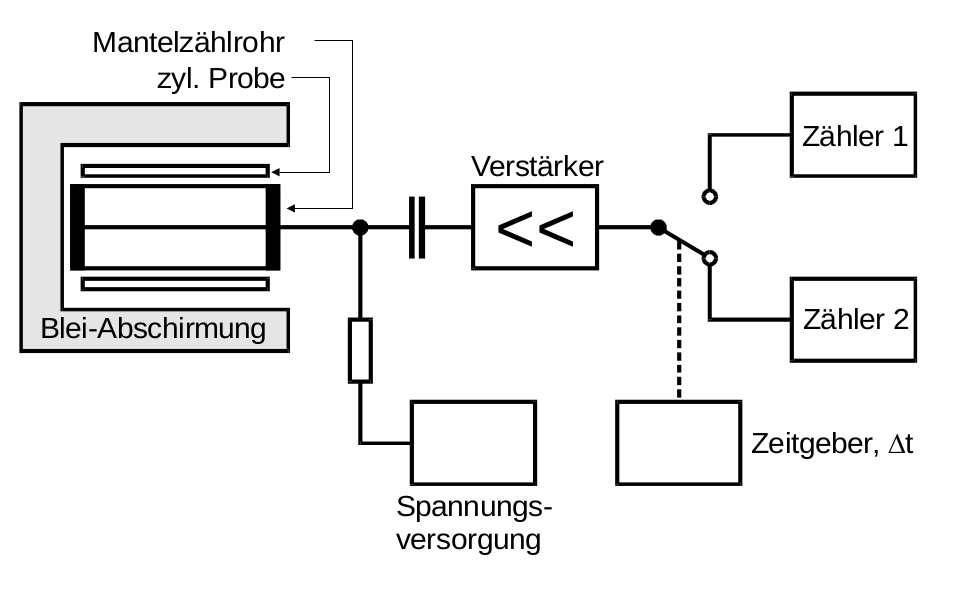
\includegraphics[width=0.8\textwidth]{Bilder/aufbau.png}
	\caption{Schematische Darstellung des Versuchsaufbaus \cite{Anleitung}.}
	\label{fig:aufbau}
\end{figure}

\begin{figure}
	\centering
	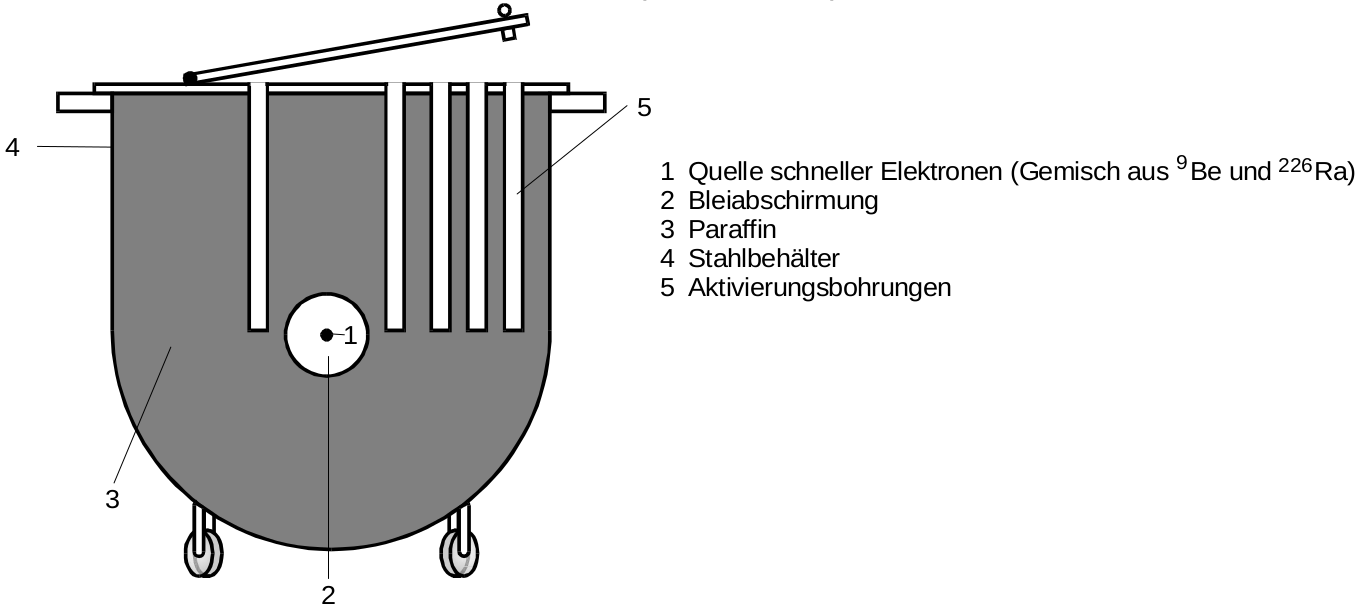
\includegraphics[width=0.8\textwidth]{Bilder/toepfchen.png}%süüüüüüüüüß, hab die datei direkt umbenannt :D
	\caption{Schematische Darstellung der Quelle zur Erzeugung radioaktiven Isotopen \cite{Anleitung}.}
	\label{fig:kochen}
\end{figure}

Der Versuchsaufbau -- wie in Abbildung \ref{fig:aufbau} dargestellt -- besteht im Wesentlichen
aus einem zerfallenden radioaktiven Isotop und einem Geiger-Müller-Zählrohr, welches die
zerfallenden Kerne misst.
Das Geiger-Müller-Zählrohr ist eine mit Gas gefüllten Röhre. Trifft ein $\beta$-
oder $\gamma$- Teilchen auf ein Gasteilchen wird dieses ionisiert und kann aufgrund einer
anliegenden Spannung an der Röhre gemessen werden.
Dabei werden die gemessenen Zerfälle pro Messzeitintervall, welches am Zeitgeber einstellbar
ist, an den Zählern 1 und 2 angezeigt. Nach jedem Messvorgang wird der Zähler umgeschaltet und
der vorherige Wert wird auf dem aktuellen Zähler überschrieben. Der Versuchsaufbau ist mit
einer Blei-Abschirmung ausgestattet um die radioaktive Strahlung abzuschirmen.

Zur Erzeugung der radioaktiven Isotope wird das Objekt in Abbildung \ref{fig:kochen} verwendet.
Hierbei werden stabile Kerne mit niederenergetischen Neutronen beschossen.
Da die Neutronen ihre Energie durch elastische Stöße an die Kerne übergeben und die maximale
Energie bei gleichen Massen der Stoßpartner erreicht wird, werden die Neutronen in einem
Paraffinmantel gebremst, bis sie die optimale Energie besitzen.
